\documentclass[runningheads]{llncs}

\usepackage{graphicx}
\usepackage[spanish]{babel}
\usepackage{tikz}
\usepackage{listings}

\begin{document}

\title{Un DSL para crear servicios REST}

\author{Enrique de la Calle Montilla y
Jorge Blázquez Saborido}
\authorrunning{F. Author et al.}
\institute{Universidad Complutense de Madrid}

\maketitle

\begin{abstract}
En este trabajo hemos diseñado e implementado un DSL para la descripción
de APIs REST que se traduce a código ejecutable en Java. El ejecutable
producido es un servidor REST funcional al que se le pueden mandar
peticiones y recibir respuestas.

Para conseguir el resultado hemos usado Eclipse y sus herramientas
asociadas: EMF, Xtext y Acceleo. Estas herramientas nos proporcionan un
entorno coherente con el que realizar ingeniería dirigida por modelos.

\keywords{Ingeniería dirigida por modelos \and DSL \and REST \and Eclipse \and EMF \and Xtext \and Acceleo \and Spark}
\end{abstract}

\section{Introducción}

% - información sobre REST
%   - un poco del contexto en el que nacen
%   - QUÉ es una API REST
% - introducción a los DSLs
% - por qué hacer un DSL para apis rest

Las \emph{APIs REST} son una arquitectura de software para el diseño
de servicios web que está muy extendida en internet desde cerca de
sus inicios. Con ella podemos diseñar la interfaz que muestra una web
al resto de la red. Esta arquitectura se fundamenta en la arquitectura
cliente-servidor, como se ve en la Figura~\ref{fig:arq-cliente-serv},
en la que el cliente y el servidor se envían mensajes. Concretamente,
en una API REST el cliente envía una petición (\emph{request}) al
servidor que este contesta en forma de respuesta (\emph{response}). Las
peticiones pueden ser de cuatro tipos, que corresponden a las
cuatro operaciones CRUD:

\newcommand\POST{\texttt{POST}}
\newcommand\GET{\texttt{GET}}
\newcommand\PUT{\texttt{PUT}}
\newcommand\DELETE{\texttt{DELETE}}

\newcommand\CREATE{\texttt{CREATE}}
\newcommand\READ{\texttt{READ}}
\newcommand\UPDATE{\texttt{UPDATE}}

\begin{itemize}
    \item \POST: es el equivalente a la operación \CREATE, con el que podemos
        crear un nuevo recurso.
    \item \GET: es el equivalente a la operación \READ, con el que podemos
        leer el contenido de un recurso ya existente.
    \item \PUT: es el equivalente a la operación \UPDATE, con el que podemos
        modificar un recurso que ya existe.
    \item \DELETE: es el equivalente a la operación \DELETE, con el que podemos
        eliminar un recurso.
\end{itemize}

\begin{figure}
\begin{center}
    \scalebox{1.3}{
        \begin{tikzpicture}[node distance = 10em]
            \node[draw, fill = red!20, minimum size = 15mm, circle] (c) {Client};
            \node[draw, fill = blue!20, minimum size = 15mm, circle, right of = c] (s) {Server};
            \draw[-stealth]
              (c.north east)
                to[out = 33, in = 90+66]
              node[above] (request) {\small request}
              node[below] {\tiny JSON/...}
              (s.north west);
            \draw[-stealth]
              (s.south west)
                to[out = 180+33, in = -33]
              node[below] (response) {\small response}
              node[above] {\tiny JSON/...}
              (c.south east);
        \end{tikzpicture}
    }
\end{center}
\caption{Arquitectura cliente servidor}
\label{fig:arq-cliente-serv}
\end{figure}

Un diseñador de una API REST cuenta con numeras bibliotecas de código
para su implementación, pero algunas veces puede ser tedioso escribir a
mano todo el código que necesita un servidor REST. Es por esto que viene
a la cabeza el concepto de \emph{DSL} (\emph{domain-specific language}),
lenguajes con un propósito muy acotado que pueden ayudarnos a automatizar
o acelerar determinadas tareas.

Este trabajo ha consistido en el diseño e implementación de un DSL para
la elaboración de APIs con la arquitectura REST. Con las herramientas
que hemos creado es posible traducir un archivo de texto que describe
la API (escrito en el DSL) a una implementación del servidor REST en
Java que hace uso de la biblioteca Spark.

En las siguientes secciones explicaremos las herramientas que hemos
usado (Sección~\ref{sc:herramientas}) durante el proceso de diseño
e implementación de nuestro DSL (Sección~\ref{sc:metodo}).
%
%En las siguientes secciones vamos a describir el proceso de diseño
%e implementación de nuestro DSL (Sección~\ref{sc:metodo}),
%además de explicar las herramientas que hemos utilizado
%(Sección~\ref{sc:herramientas}).
%
Para terminar, evaluaremos el
DSL que hemos desarrollado (Sección~\ref{sc:eval}) y concluiremos
(Sección~\ref{sc:concl}).

\section{Herramientas}
\label{sc:herramientas}

% Usamos el framework de Eclipse
% Usamos herramientas dentro de Eclipse:
% - EMF
% - xtext
% - acceleo

% TODO: citar eclipse?

El entorno de desarrollo elegido para este trabajo ha sido Eclipse, un
entorno de desarrollo integrado con soporte para modelos. Dentro de este
entorno hemos usado el \emph{Framework de Modelado de Eclipse} (EMF),
que nos da todo un abanico de herramientas para la ingeniería dirigida
por modelos. En concreto hemos usado dos de ellas: Xtext y Acceleo.

Xtext es una herramienta para el desarrollo de lenguajes de programación
y de DSLs. Gracias a su integración total con Eclipse y con el EMF,
es posible darle una sintaxis textual a nuestro metamodelo de forma
sencilla y rápida.

Acceleo es una herramienta de generación de código que también está
integrado en Eclipse y EMF. Mediante la elaboración de plantillas
podemos describir cómo queremos transformar instancias del metamodelo
a código en el lenguaje que queramos.

\section{Método}
\label{sc:metodo}

% el proceso ha comenzado con una boceto sobre cómo queríamos que fuese
% nuestro lenguaje y luego han venido unas etapas de implementación
% que han ido modificando ligeramente el lenguaje con las limitaciones
% que encontrábamos en nuestra capacidad de implementar lenguajes. Estas
% etapas han sido:
%
% - Creación del metamodelo en EMF
% - Pasar el metamodelo a XText para que nuestro DSL pueda escribirse
%   en texto.
% - (a parte) crear el proyecto de Acceleo y generar código de Spark
%   Java desde instancias del metamodelo

El proceso de desarrollo comenzó con una exploración inicial sobre
el concepto de APIs REST y de su implementación. Nos informamos de
cómo funciona esta arquitectura e investigamos diferentes bibliotecas
y lenguajes con las que se pueden implementar servidores que la siguen.
Entre los lenguajes que encontramos estaban Python y Java. A pesar de que
teníamos más experiencia en el lenguaje Python y que es un lenguaje
fácil con el que trabajar, finalmente elegimos Java como lenguaje
debido al su elevado nivel de soporte en Eclipse. Entre las bibliotecas
de Java para servidores REST que discutimos estaban \emph{Spark} y
\emph{Jersey}. Ya que Spark es una biblioteca muy sencilla con la que
no se necesita de mucho código para expresar la API REST decidimos
usarla. Elegir una biblioteca que no requiera de mucho código facilita
el trabajo en las siguientes fases de desarrollo, concretamente en la
de generación de código.

El siguiente paso fue diseñar una API REST e implementarla con
Spark Java. En nuestro caso el código de implementación
ya se nos proporcionaba y lo hemos incluido en el
Apéndice~\ref{app:codigo-inicial}. La API de ese código es la siguiente:

\begin{itemize}
    \item Las peticiones \POST\ a la dirección
        \texttt{/books} crean un nuevo recurso \emph{libro} con el autor
        y título proporcionados mediante parámetros. La respuesta
        que devuelve el servidor es el identificador del recurso.
    \item Una petición \GET\ a la dirección \texttt{/books/:id}, donde
        \texttt{:id} es el identificador de un libro, devuelve el título
        y autor del libro. Si el identificador no es válido se devolverá
        una respuesta con código de error 404.
    \item Una petición \PUT\ a la dirección \texttt{/books/:id}, donde
        \texttt{:id} es el identificador de un libro, cambia el título
        y autor del libro asignado al recurso con el identificador dado. Los
        nuevos valores de título y autor son los pasado por parámetro. Si
        el identificador no se encuentra se devuelve un error.
    \item Una petición \DELETE\ a la dirección \texttt{/books/:id}
        elimina el recurso con el identificador dado y falla si no
        se encuentra.
    \item Una petición \GET\ a la dirección \texttt{/books} devuelve todos
        los identificadores de recursos de libros.
\end{itemize}

Ahora que ya teníamos un ejemplo sobre el que trabajar nos dispusimos
a escribir en nuestro lenguaje la misma API. Como el lenguaje todavía
no existía, íbamos creando la sintaxis sobre la marcha. De esta manera
obtuvimos el primer prototipo conceptual (sin implementación) de nuestro
DSL. El resultado está en Apéndice~\ref{app:codigo-rest} y no cumple
exactamente la misma interfaz debido a las diferentes exploraciones que
hacíamos sobre la sintaxis.

\lstdefinelanguage{rest}{
    morekeywords={struct,field,post,get,put,delete,create,read,update,status,return,param,random,field,with,if,fail},
    sensitive=false,
    morestring=[b]",
}

Con esta exploración inicial ya podíamos empezar a diseñar
nuestro metamodelo.  Después de varias iteraciones (de los pasos
que vendrán a continuación) se quedó en lo que aparece en el
Apéndice~\ref{app:metamodelo}. Una vez tenemos un metamodelo ya podemos
empezar tanto con la gramática del lenguaje como con la generación de
código. Para lo primero usamos Xtext, que nos generó una gramática
por defecto. Para lo segundo usamos las plantillas de Acceleo con las
que generamos código Java que usa la biblioteca Spark.

Hemos escrito el ejemplo con el que hemos empezado esta sección en
nuestra sintaxis final (la generada por Xtext). Se puede ver en el
Apéndice~\ref{app:ejemplo-xtext}. Debe notarse que dejamos para trabajo
futuro pulir la sintaxis de nuestro lenguaje, ya que en esta fase de
desarrollo nos hemos centrado en la semántica y en que la generación
de código funcione correctamente.

La generación de código con Acceleo funciona con una serie de
plantillas, como se ve en la Figura~\ref{fig:acceleo-files}. Cada una
de ellas tiene una función específica, para así tener un código
de generación modular. En la Figura~\ref{fig:gen-read} mostramos la
plantilla de generación de código de la operación \READ. El código generado
es sencillo:

\begin{itemize}
    \item Primero se busca el recurso solicitado con el identificador dado.
    \item Si el recurso se encuentra se guardará el nombre de cada atributo
        en variables locales para que puedan ser usados en otras
        operaciones o en la respuesta.
    \item Si el recurso no se encuentra se devolverá la respuesta de fallo.
\end{itemize}

\begin{figure}
    \centering
    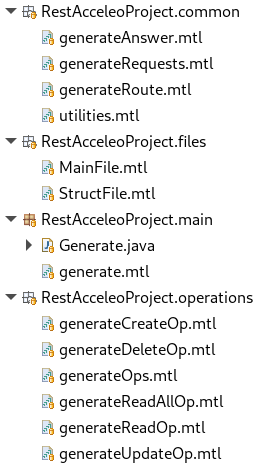
\includegraphics[width=0.4\textwidth]{acceleo-files}
    \caption{Plantillas de Acceleo}
    \label{fig:acceleo-files}
\end{figure}

\begin{figure}
    \centering
    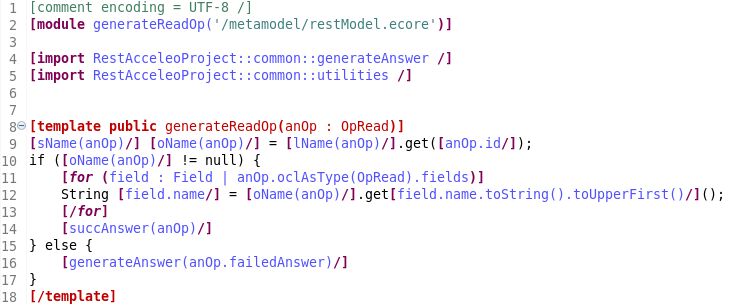
\includegraphics[width=\textwidth]{generateReadOp}
    \caption{Generación de código de la operación \READ}
    \label{fig:gen-read}
\end{figure}

\section{Evaluación}
\label{sc:eval}

En esta sección se procede a escribir el flujo de trabajo necesario para generar un proyecto ejecutable de servidor REST.

Como paso previo, hemos visto necesario registrar nuestro metamodelo dinámicamente como se indica en \url{https://github.com/martin-fleck/momot/issues/14\#issuecomment-327720552} 

En primer lugar, si se quiere utilizar un editor de los ficheros \textit{.rest}, es necesario ejecutar el proyecto \textit{xtextREST.ide} como una aplicación de Eclipse. Esta acción abrirá un IDE, en el cual podremos crear un proyecto vacío con un fichero \textit{.rest}. Se ha codificado el fichero \textit{datamodel.rest} que se puede encontrar en la carpeta \textit{files} en la raíz del directorio de entrega.

En segundo lugar, es necesario convertir dicho fichero en una instancia dinámica \textit{.xmi}. Para ello se hace uso de una pequeña herramienta proporcionada en el proyecto \textit{xtextREST}, dentro de \textit{src/converter}. Dentro de este paquete hay un fichero \textit{Main.java} que al ser ejecutado como aplicativo Java, abrirá un buscador de archivos. Tras localizar el archivo \textit{datamodel.rest} y aceptar, un nuevo fichero en la misma localización llamado \textit{datamodel.xmi} aparece, el cual la es instancia dinámica que utilizaremos a partir de ahora.

Como paso opcional, es posible convertir esta instancia dinámica en un fichero \textit{.ecore}. Si se desea realizar esta transformación, se debe abrir el proyecto \textit{AtlM2M}. La ejecución de este proyecto depende de cuatro parámetros: El metamodelo de entrada MM, el metamodelo de salida MM2, el modelo de entrada IN y el modelo de salida OUT1. Tanto como para el metamodelo MM como para MM2, se ha elegido el metamodelo \textit{restModel}, ya que la transformación es una referencia al propio metamodelo. Para el modelo de entrada, se ha elegido \textit{datamodel.xmi} y para la salida, un nuevo fichero \textit{datamodel.ecore}. Tras ejecutar este proyecto, el fichero resultante de la transformación \textit{datamodel.ecore} es accesible desde el editor de modelos \textit{.ecore} de Eclipse.

En tercer lugar, se procede a la transformación de la instancia dinámica en un proyecto Java. Se ha creado un proyecto vacío \textit{RESTServer} con las librerías necesarias incluidas y con una carpeta src. Posteriormente se ejecuta el proyecto \textit{RestAcceleoProject} con los parámetros necesarios, en concreto destacar que el \textit{Target} de salida debe ser la carpeta \textit{src} del proyecto vacío. Llegados a este punto, se deben haber creado dos archivos en dicha carpeta, uno llamado \textit{Book.java} que incluye el contenido del struct \textit{Book} y otro fichero \textit{Main.java}. Ahora es posible ejecutar dicho fichero como aplicación Java.

Por último se ha probado el proyecto resultante \textit{RESTServer} ya poblado de código. Al ejecutarlo, se inicia un servidor REST en el puerto :4567. Con la consola de comandos, la primera petición realizada ha sido:

\texttt{\$ curl -X POST "http://localhost:4567/books?author=FIbanez\&title=SuperHumor"}

Esta petición debería ejecutar el código de request Post, que a su vez realiza la operación de inserción de un nuevo libro con los parámetros autor y título. El resultado es:

\texttt{\$ 1081732467}

que corresponde al id del libro añadido. Este id se utilizará en las siguientes llamadas.

La siguiente petición probada ha sido GET, que debe leer el libro con id pasado a través de la ruta.

\texttt{\$ curl -X GET "http://localhost:4567/books/1081732467"}

el resultado es:

\texttt{\$Title: SuperHumor, Author: FIbanez}

Si quisieramos leer un libro que no existe como:

\texttt{\$ curl -X GET "http://localhost:4567/books/1"}

el resutado es simplemente

\texttt{\$ error}

En caso de querer editar el libro añadido, se procede a utilizar la request PUT, que a su vez está vinculada a la operación UPDATE en el DSL. Esta petición incluye los parámetros que queremos editar como parámetros de la url.

\texttt{\$ curl -X PUT "http://localhost:4567/books/1081732467?author=Escobar"}

como resultado obtenemos el mensaje definido en el DSL:

\texttt{\$ Book with id 1081732467 updated}

Vamos a comprobar si los cambios se han guardado:

\texttt{\$ curl -X GET "http://localhost:4567/books/1081732467"}

\texttt{\$Title: SuperHumor, Author: Escobar}

Por último se ha evaluado la request DELETE, que a su vez tiene una operación de borrado asociada.

\texttt{\$ curl -X DELETE "http://localhost:4567/books/1081732467"}

resultado:

\texttt{\$ Book with id 1081732467 deleted}

y ahora al intentar acceder al libro borrado con

\texttt{\$ curl -X GET "http://localhost:4567/books/1081732467"}

se obtiene otro mensaje de error.

% hablar de las pruebas que le hemos hecho al código

%\section{Trabajo relacionado}

% quizá quitarlo xD

\section{Conclusiones}
\label{sc:concl}

El resultado de este trabajo es el diseño e implementación de un DSL
para describir APIs REST. Hemos implementado un generador de código que
traduce el DSL a un servidor ejecutable que recibe peticiones y devuelve
las respuestas especificadas por el usuario.

Para conseguir ello hemos usado Eclipse, concretamente el entorno EMF
y las herramientas que se utilizan con él: EMF, Xtext y Acceleo. En
conjunto, hemos usado un entorno de desarrollo para realizar ingeniería
dirigida por modelos.

Planteamos distintas extensiones o modificaciones a nuestro lenguaje:

\begin{itemize}
    \item Modificar la sintaxis en Xtext para no tener que escribir tantos
        corchetes y tantas palabras claves.
    \item Ampliar el DSL para poder escribir expresiones y sentencias
        de Java.
    \item Mejorar las restricciones para detectar más casos de código
        erróneo.
\end{itemize}

\newpage

\appendix
\section{Código inicial}
\label{app:codigo-inicial}

\begin{center}
\begin{lstlisting}[language=java, basicstyle = \footnotesize, xleftmargin=-.1\textwidth]
import static spark.Spark.*;
import java.util.*;
import spark.Request;
import spark.Response;
import spark.Route;
// A simple RESTful example showing howto create, get, update and delete
// book resources.
public class Books {
  // Map holding the books
  private static Map < String, Book > books = new HashMap < String, Book > ();
  public static void main(String[] args) {
    // Creates a new book resource, will return the ID to the created resource
    // author and title are sent as query parameters
    // e.g. /books?author=Foo&title=Bar
    post(new Route("/books") {
      Random random = new Random();
      @Override
      public Object handle(Request request, Response response) {
        String author = request.queryParams("author");
        String title = request.queryParams("title");
        Book book = new Book(author, title);
        int id = random.nextInt(Integer.MAX_VALUE);
        books.put(String.valueOf(id), book);
        response.status(201); // 201 Created
        return id;
      }
    });
    // Gets the book resource for the provided id
    get(new Route("/books/:id") {
      @Override
      public Object handle(Request request, Response response) {
        Book book = books.get(request.params(":id"));
        if (book != null) {
          return "Title: " + book.getTitle() + ", Author: " + book.getAuthor();
        } else {
          response.status(404); // 404 Not found
          return "Book not found";
        }
      }
    });
    // Updates the book resource for the provided id with new information
    // author and title are sent as query parameters
    // e.g. /books/<id>?author=Foo&title=Bar
    put(new Route("/books/:id") {
      @Override
      public Object handle(Request request, Response response) {
        String id = request.params(":id");
        Book book = books.get(id);
        if (book != null) {
          String newAuthor = request.queryParams("author");
          String newTitle = request.queryParams("title");
          if (newAuthor != null) {
            book.setAuthor(newAuthor);
          }
          if (newTitle != null) {
            book.setTitle(newTitle);
          }
          return "Book with id '" + id + "' updated";
        } else {
          response.status(404); // 404 Not found
          return "Book not found";
        }
      }
    });
    // Deletes the book resource for the provided id
    delete(new Route("/books/:id") {
      @Override
      public Object handle(Request request, Response response) {
        String id = request.params(":id");
        Book book = books.remove(id);
        if (book != null) {
          return "Book with id '" + id + "' deleted";
        } else {
          response.status(404); // 404 Not found
          return "Book not found";
        }
      }
    });
    // Gets all available book resources (id's)
    get(new Route("/books") {
      @Override
      public Object handle(Request request, Response response) {
        String ids = "";
        for (String id: books.keySet())
          ids += id + " ";
        return ids;
      }
    });
  }
}
\end{lstlisting}
\end{center}

\newpage

\section{Primer prototipo de API REST}
\label{app:codigo-rest}

\begin{lstlisting}[language=rest, basicstyle=\footnotesize]
struct Page {
  field num;
}

struct Book {
  field author;
  field title;
  field pageId;
}

post "book" {
  param author;
  param title;
  param pageId;
  random id;
  create Book(author: author, title: title, pageId: pageId) with id;
  status 201;
  return "{id}";
}

get "books" id {
  read Book(author, title, pageId) with id if fail {
    status 404;
    return "Book not found"
  };
  return "Title: {title}, Author: {author}";
}

get "books" id "name" {
  read Book(author, title, pageId) with id if fail {
    status 404;
    return "Book not found"
  };
  return title;
}

put "books" id {
  param newAuthor;
  param newTitle;
  update Book(author: newAuthor, title: newTitle) with id if fail {
    status 404;
    return "Book not found";
  };
  return "Book with id '{id}' updated";
}
\end{lstlisting}

\newpage

\section{Metamodelo del DSL}
\label{app:metamodelo}

\begin{center}
    \rotatebox{90}{\scalebox{0.5}{\input{restModel.pdf_tex}}}
\end{center}

\newpage
\section{Código con sintaxis final}
\label{app:ejemplo-xtext}

\begin{center}
\begin{lstlisting}[basicstyle = \scriptsize]
RestSystem
{
    requests {
        RePost {
            succAnswer post

            route Route{ 
                segments{
                    Segment{
                        value books
                    }
                } 
            }

            operations {
                OpCreate {
                    failedAnswer fail
                    struct Book
                    fieldsets {
                        FieldSet author {
                            value author
                        },
                        FieldSet title {
                            value title
                        }
                    }
                }
            }

            parameters {
                Parameter author,
                Parameter title
            }
        },

        ReGet {
            succAnswer read

            route Route {
                segments {
                    Segment {
                        value books
                    },
                    Segment {
                        value ':id'
                    }
                } 
            }

            operations {
                OpRead {
                    id 'id'
                    failedAnswer fail
                    struct Book
                    fields ("Book.author", "Book.title")    
                }
            }
        },

        ReDelete {
            succAnswer del

            route Route { 
                segments {
                    Segment {
                        value books
                    },
                    Segment{
                        value ':id'
                    }
                } 
            }

            operations {
                OpDelete {
                    id 'id'
                    failedAnswer fail
                    struct Book
                }
            }
        },

        RePut {
            succAnswer up

            route Route { 
                segments {
                    Segment {
                        value books
                    },
                    Segment {
                        value ':id'
                    }
                } 
            }

            operations {
                OpUpdate {
                    id 'id'
                    failedAnswer fail
                    struct Book
                    fieldsets {
                        FieldSet author{
                            value author
                        },
                        FieldSet title{
                            value title
                        }
                    }
                }
            }

            parameters {
                Parameter author,
                Parameter title
            }
        }
    }

    structs {
        Struct Book {
            fields {Field author, Field title}
        }
    }

    answers {
        Answer post {
            status 201
            return "id"
        },
        Answer read {
            status 200
            return '"Title: " + title + ", Author: " + author'
        },
        Answer fail {
            status 404
            return '"error"'
        },
        Answer up {
            status 200
            return '"Book with id " + id + " updated"'
        },
        Answer del {
            status 200
            return '"Book with id " + id + " deleted"'
        }
    } 
}
\end{lstlisting}
\end{center}

\end{document}
